% \chapter{Long Title}{Short Title}
% The Long Title will appear on the first page of the chapter.
% The Short Title will appear in the table of contents.
% If the Long Title isn't all that long, you can just call
% \chapter{Long Title}{} and the same title will appear in
% both places.


\chapter{Convergence of Pad\'e approximants}{}

Here we, hear ye, discuss the convergence of rational approximations to the Stieltjes transform. Namely, the Pad\'e approximants to the moment series are defined and convergence to the Stieltjes transform is proved under certain restrictions.

\section{The Markov and Hamburger transforms}

Let $\mu$ be a Borel measure with finite moments $c_k = \int_{-\infty}^\infty p^k d\mu$. 

\begin{definition}
  The complex function $g$ defined by
  \[
    g(z) = \int_{-\infty}^\infty\frac{d\mu}{1+zp}
  \]
  is called the Markov (Hamburger resp.) transform of $\mu$ when $\mu$ has bounded (unbounded resp.) support.
\end{definition}

It is worth noting at the outset that $g(z)$ is defined at least for non-real $z$. To see this we note that if $\im z \neq 0$,
\begin{align*}
  \frac1{|1 + zp|} 
  &= \frac{|1/z|}{|\frac1z + p|} \\
  &\leq \frac{|1/z|}{|\im \frac1z|} \\
  &= \frac{|\overline{z}|/|z|^2}{|\im \overline{z}|/|z|^2} \\
  &= \frac{|z|}{|\im z|}
\end{align*}
which gives the bound
\begin{equation}
  |g(z)| 
  \leq \int_{-\infty}^\infty \frac{|z|}{|\im z|} d\mu(p) 
  = \frac{|z|}{|\im z|}c_0
\end{equation}

Since the integrand has a singularity only when $p = -1/z$ a Markov transform must converge in some neighborhood of zero. This cannot be said in general for a Hamburger transform. 

\begin{remark}
  The bound above has a useful geometric interpretation. For starters we note that,
  \[
    \frac{|\im z|}{|z|} = |\sin(\arg z)|,
  \]
  which can be seen by considering the right triangle formed by the points $0$, $z$, and $\re z$. Thus this bound essentially depends on the angle of separation between $z$ and the real line. 
\end{remark}

\begin{proposition}
  The function $g(z)$ is analytic on the upper and lower half planes $\im z \neq 0$.
\end{proposition}

\begin{proof}
  Let $z, w$ be complex numbers with non-zero imaginary part. We have
  \begin{align*}
    g(w) - g(z)
    &= \int_{-\infty}^\infty \frac{1}{1 + wp} - \frac1{1 + zp}d\mu(p) \\
    &= \int_{-\infty}^\infty \frac{(1 + zp) - (1 + wp)}{(1 + wp)(1 + zp)}d\mu(p) \\
    &= (w - z) \int_{-\infty}^\infty \frac{-p}{(1 + wp)(1 + zp)}d\mu(p).
  \end{align*}
  Thus it seems
  \[
    \lim_{w \rightarrow z} \frac{g(w) - g(z)}{w - z} = \int_{-\infty}^\infty \frac{-p}{(1+zp)^2}d\mu(p).
  \]
  To be precise we may justify the interchange of limit and integral here by dominated convergence. Recall that it suffices to find an integrable function $h : \RR \to \CC$ such that, for any $w$ in a neighborhood of $z$,
  \[
    \left|\frac{-p}{(1 + wp)(1 + zp)}\right| \leq h(p) \qquad \hbox{for all $p \in \RR$}.
  \]
  It should be noted that our particular dominating function $h(p)$ is somewhat arbitrary, and not a sharp bound. By the previously discussed bound we have,
  \[
    \left|\frac{-p}{(1 + wp)(1 + zp)}\right| \leq |p|\frac{|wz|}{|\im w ~\im z|}.
  \]
  Furthermore $|w|/|\im w|$ is clearly continuous on the half planes, so in some neighborhood of 
  \[
    |p|\frac{|wz|}{|\im w ~\im z|} \leq |p|\left(\frac{|z|^2}{|\im z|^2} + \epsilon\right)
  \]
  for an arbitrary $\epsilon > 0$. Finally, we note that the right hand dominating function above is integrable since $\mu$ has finite moments: 
  \[
    \int_{-\infty}^\infty |p| d\mu \leq \int_{-\infty}^\infty \frac12(p^2 + 1) ~d\mu = c_2 + c_0
  \]
\end{proof}

\begin{remark}
  Since $\mu$ is a real measure, $g(z)$ commutes with conjugation,
  \[
    g(\bar z) = \int_\infty^\infty\frac{d\mu}{1+\bar zp} = \overline{\int_\infty^\infty\frac{d\mu}{1+zp}} = \overline{g(z)}.
  \]
  For this reason, although $g(z)$ is defined for all non-real $z$, we will only concern ourselves with its values on the upper half plane $\im z > 0$ going forward. In chapter 3 we should restrict our sample points to the upper half plane, since samples in the lower half may be redundant.
\end{remark}


When $z$ is a real number $g(z)$ may not converge. In particular $g(z)$ does not converge when $z = -1/p$ for some $p$ in the support of $\mu$ \pn.  Thus if $\mu$ has bounded support $g$ converges in a neighborhood of $0$. On the other hand if $\mu$ has unbounded support $g(0)$ is not defined. However — as we will see — even in the Hamburger transform case, a formal series expansion at $z = 0$ holds valuable information. The results of this section are described in detail in section 5.6 of (Baker) \cn

By a geometric series expansion,
\[
  \frac1{1 + zp} = \sum_{k = 0}^\infty {(-z)}^k p^k 
\]
when $|zp| < 1$. This suggests the connection between $g(z)$ and the moment sequence ${(c_k)}_{k \in \NN_0}$. Indeed, at least formally,
\begin{align*}
  \int_\infty^\infty\frac{d\mu}{1+zp}
  &= \int_\infty^\infty \sum_{k = 0}^\infty {(-z)}^k p^k ~d\mu \\
  &= \sum_{k = 0}^\infty {(-z)}^k \int_\infty^\infty p^k ~d\mu \\
  &= \sum_{k = 0}^\infty c_k{(-z)}^k.
\end{align*}
In the Markov case we have a positive radius of convergence. But even in the Hamburger case, there is a sense in which this assymptotic expansion holds ``non-tangentially''.

Non-tangential convergence at $z = 0$ is, as the name implies, convergence along curves not tangent to the real line at $0$. More precisely, one defines a ``wedge domain''
\[
  \Gamma_\delta = \{\delta \leq \arg z \leq \pi - \delta\}
\]
\begin{figure}
  \centering
  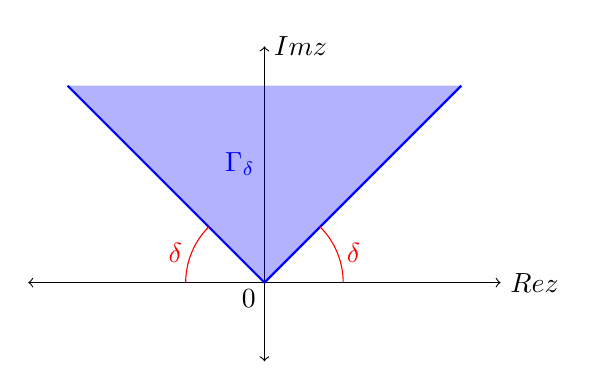
\begin{tikzpicture}[wedge/.style={blue, fill=blue, fill opacity = 0.3}, angle/.style={red}, axis/.style={<->,black}]
    %draw axes
    \draw[axis] (-3,0) -- (3,0) node[anchor=west]{$\text{Re} z$};
    \node at (-.2,-.2) {$0$};
    \draw[axis] (0,-1) -- (0,3) node[anchor=west]{$\text{Im} z$};
    %draw wedge
    \fill[wedge] (0, 0) -- (-2.5, 2.5) -- (2.5,2.5) -- cycle;
    \draw[thick, blue] (-2.5, 2.5) -- (0,0) -- (2.5,2.5);
    \node[left, blue] at (0,1.5) {$\Gamma_\delta$};
    %draw angle
    \def\ra{.07};
    \draw[red] (1,0) arc (0:45:1) node[midway, right]{$\delta$};
    \draw[red] (-1,0) arc (180:135:1)node[midway, left]{$\delta$};
  \end{tikzpicture}
  \caption{A wedge domain}\label{fig:wedge}
\end{figure}
in which curves approach $0$ with an angle at least $\delta$ from the real line.

\begin{definition} (Non-tangential convergence and assymptotic expansion)
  We say $h(z) \rightarrow 0$ non-tangentially as $z \rightarrow 0$ if, for any $\delta > 0$, the limit 
  \[
    \lim_{z \rightarrow 0} h(z) = 0
  \]
  holds for $z$ in the $\Gamma_\delta$. If a formal power series $\sum_{k=0}^\infty a_k z^k$ and a function $g(z)$ are such that for all $n\in \NN_0$,
  \[
    g(z) = \sum_{k = 0}^{n-1} c_k{(-z)}^k + z^n h_n(z)
  \]
  where the trailing terms $h_n(z)$ converge to $0$ non-tangentially as $z \rightarrow 0$, we say that $\sum_{k=0}^\infty a_k z^k$ is an assymptotic expansion of $g(z)$. We use the notation
  \[
    g(z) \simeq \sum_{k=0}^\infty a_k z^k
  \]
  for assymptotic expansions.
    % If for any $\delta > 0$ the limit $g(z) \rightarrow L$ holds 
\end{definition}

While $g(z)$ does not generally converge at $z = 0$, in a non-tangential sense the afformentioned assymptotic expansion holds:
\begin{proposition}
  \begin{enumerate}
    \item If $\mu$ has bounded support
    \[
      g(z) = \sum_{k = 0}^\infty c_k{(-z)}^k
    \]
    in a neighboorhood of $z=0$.
    \item For all $n \in \NN_0$
    \begin{equation}
      g(z) = \sum_{k = 0}^{n-1} c_k{(-z)}^k + z^n h_n(z) \label{assexp}
    \end{equation}
    where $h_n$ is such that $\lim_{z \rightarrow 0} h_n(z) = 0$ non-tangentially.
  \end{enumerate}
\end{proposition}

\begin{proof}
  We first note that 
  \[
    \sum_{k=0}^{n} c_k {(-z)}^k 
    = \sum_{k=0}^{n} \int_{-\infty}^\infty {(-zp)}^k d\mu
    % = \int_{-\infty}^\infty \sum_{k=0}^{n} (-zx)^k d\mu
    = \int_{-\infty}^\infty \frac{1 - {(-zp)}^{n+1}}{1 + zp} d\mu
  \]
  and so
  \begin{align*}
    h_n(z) = \frac1{z^n}\left\{g(z) - \sum_{k=0}^{n} c_k {(-z)}^k\right\}
    &= \int_{-\infty}^\infty \frac{zp^{n+1}}{1 + zp}d\mu.
  \end{align*}
  It remains to determine if and in what sense this trailing term $h_n(z)$ vanishes at the origin. 

  As expected in the case when $\mu$ has bounded support, $h_n(z)$ exists in a neighborhood of $0$ and vanishes as $z \rightarrow 0$ in this neighboorhood. Thus the assymptotic expansion~\ref{assexp} is the Taylor expansion: The Markov transform is analytic at the origin.

  When $\mu$ has unbounded support and $h_n(z)$ may not be well defined on the real line, so we must weaken our result to non-tangential convergence. If $z \in \Gamma_\delta$ then we have the following inequalities for any $p \in \RR$,
  \[
    |p - z| \geq |p| \sin \delta 
    \quad\text{and} \quad
    |p - z| \geq |p| \sin \delta.
  \]
  We will show that
  \[
    \lim_{z \rightarrow 0} h_{2n}(z) = 0, \quad z \in \Gamma_\delta
  \]
  from which the corresponding limit for odd orders will immediately follow from the relation
  \[
    h_{2n-1}(z)
    = zh_{2n}(z) + c_{2n}z^{2n}.
  \] 
  Here for the sake of convenience we define $w = -\frac1z$, following a more classical approach. Note that $|w| = \frac1{|z|}$ and if $z$ is in the wedge $\Gamma_\delta$ then so is $w$. Now 
  \begin{align*}
    |h_{2n}(z)| 
    &\leq \int_{-\infty}^\infty \frac{|p|^{2n+1}}{|p - w|}d\mu \\
    &\leq \frac{|z|}{\sin \delta} \int_{|p| \leq A} |p|^{2n+1} d\mu
    + \frac1{\sin \delta} \int_{|p| \geq A} p^{2n} d\mu \\
    &\leq \frac{2|z| A^{2n+2}}{\sin \delta}
    + \frac1{\sin \delta} \int_{|p| \geq A} p^{2n} d\mu
  \end{align*}
  Thus 
  \[
    \lim_{z \rightarrow 0} |h_{2n}(z)| \leq \frac1{\sin \delta} \int_{|p| \geq A} p^{2n} d\mu, \quad z \in \Gamma_\delta.
  \]
  Since $A$ is arbitrary and the integral $\int p^{2n} d\mu = c_{2n}$ is convergent we are done.
\end{proof}

\begin{remark}
  An interesting connection — which I don't know enough about to discuss yet — is begining to be revealed here between moment problems and analytic functions on the upper half plane (in particular, their behaviour near the real boundary). This leads us to the notion of interpolation problems \cn.
\end{remark}

Evidently the assymptotic series expansion $g(z) \simeq \sum_{k=0}^\infty c_k {(-z)}^k$ is generally formal, having zero radius of convergence except in the Markov case. However as we will see in the next section, rational functions constructed from this formal series exist which approximate $g(z)$ on the upper half plane $\{\text{Im} z > 0\}$.

Finally we prove two propositions regarding the Hamburger transform of a RT projection. Let $\omega \in S^{n-1}$ be fixed and consider
\[
  g(z) = \int_\infty^\infty \frac{R(\omega, p)}{1 + zp} dp
\]
for some function $f: \RR^n \to \RR$. 
\begin{definition}
  The multivariate Markov (Hamburger resp.) transform of a borel measure $\mu$ on $\RR^n$ of bounded (unbounded resp.) support is defined by
  \[
    g(y) = \int_{\RR^n} \frac{d\mu(x)}{1 + \langle x, y\rangle} \simeq \sum_{\alpha \in \NN_0^n} c_\alpha(-y)^\alpha
  \]
  when $\mu$ has finite moments $c_\alpha = \int_{\RR^n} x^\alpha d\mu$.
\end{definition}
% \begin{proposition}
%   The Hamburger transform of the Radon transform of a function $f$ is 
%   \[
%     \int_{-\infty}^\infty \frac{R_f(\omega, p)}{1 + zp} dp = \int_{\RR^n} \frac{f(x)}{1 + z\langle x, \omega \rangle} dx
%   \]
% \end{proposition}

% \begin{proposition}
  
% \end{proposition}
By applying the slice theorem, with $F(p) = {(1+zp)}^{-1}$ we see that the Hamburger transform of a projection can be represented by a similar multivariable integral of $f$ over $\RR^n$.
\[
  \int_{-\infty}^\infty \frac{R_f(\omega, p)}{1 + zp} dp = \int_{\RR^n} \frac{f(x)}{1 + z\langle x, \omega \rangle} dx
\]
Similarly the GRT slice theorem with $F(p) = {(1 + zp)}^{-1}$ is
\[
  \int_{-\infty}^\infty \frac{GR_f(\omega, p) w(p)}{1 + zp} dp = \int_{\RR^n} \frac{f(x)w_n(x)}{1 + z\langle x, \omega \rangle} dx.
\]


\section{Pad\'e approximants}

In this section we recall the necessary definitions and results. Then we will prove some new results to be applied to the Gaussian Radon transform later.

\begin{definition}[Classical definition of Pad\'e approximants]
  The Pad\'e approximant to a (possibly formal) power series 
  \[
    R^{[L/M]}(z) \simeq \sum_{k=0}^\infty c_k z^k
  \]
  is a rational function with nummerator (denominator resp.) degree at most $L$ ($M$ resp.), with series equal to $\sum_{k=0}^N c_k z^k + O(z^{N+1})$ up to as high an order $N$ as possible. 
\end{definition}

Let
\[
  R^{[L/M]}(z) = \frac{P^{[L/M]}(z)}{Q^{[L/M]}(z)} = \frac{a_L z^L + \cdots + a_1z + a_0}{b_M z^M + \cdots + b_1z + b_0}.
\]
Notice that in general there is a negligable constant common factor between the numerator and denominator, so that with the remaining $L+M+1$ free parameters, we expect an order of accuracy of up to $L+M+1$ constraints, $c_0, c_1, \ldots, c_{L+M}$. Thus we define the $[L/M]$ Pad\'e approximant by the condition,
\begin{equation}
  \label{eq:BPade}
  \frac{P^{[L/M]}(z)}{Q^{[L/M]}(z)} = \sum_{k=0}^{L+M} c_k z^k + O\left(z^{L+M+1}\right).
\end{equation}
It is helpful to consider the related, and necessary condition
\begin{equation}
  \label{eq:CPade}
  P^{[L/M]}(z) = Q^{[L/M]}(z)\left(\sum_{k=0}^{L+M} c_k z^k\right) + O\left(z^{L+M+1}\right).
\end{equation}
In the classical theory of Pad\'e approximants (\ref{eq:CPade}) was often taken as a definition. It is always possible to find polynomials of the required degree satisfying this second condition, however they do not necessarily attain the degree of accuracy required by the first. We follow Baker, defining $R^{[L/M]}(z)$ by (\ref{eq:BPade}), provided such a rational function exists.

\begin{definition}[Baker's definition of Pad\'e approximants]
  The Pad\'e approximant $R^{[L/M]}$ to a (possibly formal) power series is a the unique rational function with nummerator (denominator resp.) degree at most $L$ ($M$ resp.) satisfying the condition (\ref{eq:BPade}). If no such rational function exists we say the Pad\'e approximant does not exist.
\end{definition}

Here we note that a sufficient condition for the equivalence of the two definitions, and hence for the existence of the Pad\'e approximant by Baker's definition is that $b_0 = Q^{L/M}(0) \neq 0$. 

Equating coeffictients of $z^k$, $k = 0, 1, \ldots, L+M$ in (\ref{eq:CPade}) gives two linear systems
\begin{align*}
  a_0 &= b_0c_0 \\
  a_1 &= b_1c_0 + b_0c_1 \\
  &\vdots \\
  a_L &= b_L c_0 + b_{L-1}c_1 + \cdots + b_0c_L
\end{align*}
and,
\begin{align*}
  0 &= b_{M}c_{L-M+1} + b_{M-1}c_{L-M+2} + \cdots + b_0c_{L+1} \\
  0 &= b_{M}c_{L-M+2} + b_{M-1}c_{L-M+3} + \cdots + b_0c_{L+2} \\
  &\vdots \\
  0 &= b_{M}c_L + b_{M-1}c_{L+1} + \cdots + b_0c_{L+M}
\end{align*}
where for convenience we set $c_k = 0$ for $k < 0$. The first system shows the numerator $P^{[L/M]}$ is determined by the denominator $Q^{[L/M]}$. From the second system we can derive a determinantal formula for $Q^{[L/M]}$. Augmented with the desired definition, 
\[
  Q^{[L/M]}(z) = b_M z^M + b_{M-1}z^{M-1} + \cdots + b_0
\]
the system can be written in the form
\[
  \begin{pmatrix}
    0 \\ 0 \\ \vdots \\ 0 \\ Q^{[L/M]}(z)
  \end{pmatrix}
  =
  \begin{pmatrix}
    c_{L-M+1} & c_{L-M+2} & \cdots & c_{L+1} \\
    c_{L-M+2} & c_{L-M+3} & \cdots & c_{L+2} \\
    \vdots & \vdots & \ddots & \vdots \\
    c_{L} & c_{L+1} & \cdots & c_{L+M} \\
    z^M & z^{M-1} & \cdots & 1
  \end{pmatrix}
  \begin{pmatrix}
    b_M \\ b_{M-1} \\ \vdots \\ b_1 \\ b_0
  \end{pmatrix}
\]
Solving for $b_0$ by Cramer's Rule we get,
% \[
%     b_0 = 
%     \frac{
%         \left|
%         \begin{matrix}
%             c_{L-M+1} & c_{L-M+2} & \cdots & c_L & 0 \\
%             c_{L-M+2} & c_{L-M+3} & \cdots & c_{L+1} & 0 \\
%             \vdots & \vdots & \ddots & \vdots & \vdots \\
%             c_L & c_{L+1} & \cdots & c_{L+M-1} & 0 \\
%             z^M & z^{M-1} & \cdots & z & Q^{[L/M]}(z)
%         \end{matrix}
%         \right|
%     }{
%         \left|
%         \begin{matrix}
%             c_{L-M+1} & c_{L-M+2} & \cdots & c_{L+1} \\
%             c_{L-M+2} & c_{L-M+3} & \cdots & c_{L+2} \\
%             \vdots & \vdots & \ddots & \vdots \\
%             c_{L} & c_{L+1} & \cdots & c_{L+M} \\
%             z^M & z^{M-1} & \cdots & 1
%         \end{matrix}
%         \right|
%     }
% \]

% \[
%     b_0 = 
%     \frac{
%         \left|
%         \begin{matrix}
%             c_{L-M+1} & c_{L-M+2} & \cdots & c_L \\
%             c_{L-M+2} & c_{L-M+3} & \cdots & c_{L+1} \\
%             \vdots & \vdots & \ddots & \vdots  \\
%             c_L & c_{L+1} & \cdots & c_{L+M-1} 
%         \end{matrix}
%         \right| Q^{[L/M]}(z)
%     }{
%         \left|
%         \begin{matrix}
%             c_{L-M+1} & c_{L-M+2} & \cdots & c_{L+1} \\
%             c_{L-M+2} & c_{L-M+3} & \cdots & c_{L+2} \\
%             \vdots & \vdots & \ddots & \vdots \\
%             c_{L} & c_{L+1} & \cdots & c_{L+M} \\
%             z^M & z^{M-1} & \cdots & 1
%         \end{matrix}
%         \right|
%     }
% \]

\[
  b_0
  \left|
  \begin{matrix}
    c_{L-M+1} & c_{L-M+2} & \cdots & c_{L+1} \\
    c_{L-M+2} & c_{L-M+3} & \cdots & c_{L+2} \\
    \vdots & \vdots & \ddots & \vdots \\
    c_{L} & c_{L+1} & \cdots & c_{L+M} \\
    z^M & z^{M-1} & \cdots & 1
  \end{matrix}
  \right|
  =
  \left|
  \begin{matrix}
    c_{L-M+1} & c_{L-M+2} & \cdots & c_L \\
    c_{L-M+2} & c_{L-M+3} & \cdots & c_{L+1} \\
    \vdots & \vdots & \ddots & \vdots  \\
    c_L & c_{L+1} & \cdots & c_{L+M-1} 
  \end{matrix}
  \right| 
  Q^{[L/M]}(z)
\]
The LHS is clearly a polynomial, and nonzero if the RHS minor is nonzero. Thus if the Hankel determinant
\[
  \left|
  \begin{matrix}
    c_{L-M+1} & \cdots & c_L \\
    \vdots & \ddots & \vdots  \\
    c_L & \cdots & c_{L+M-1} 
  \end{matrix}
  \right| 
\]
is nonzero, then up to the afformentioned constant factor,
\begin{equation}
  Q^{[L/M]}(z) = 
  \left|
  \begin{matrix}
    c_{L-M+1} & \cdots & c_{L+1} \\
    \vdots & \ddots & \vdots \\
    c_{L} & \cdots & c_{L+M} \\
    z^M & \cdots & 1
  \end{matrix}
  \right| 
  \label{eq:Qdet}
\end{equation}
By convention we normalize $R^{[L/M]}(z)$ so that $b_0 = Q^{[L/M]}(0) = 1$. 

Since the Hankel determinants give a useful form for expressing some conditions of interest we will difine $H(n,m)$ to be the determinant of the $(m + 1) \times (m + 1)$ Hankel matrix starting with $c_n$,
\[
  H(n,m) :=
  \left|
  \begin{matrix}
    c_{n} & \cdots & c_{n+m} \\
    \vdots & \ddots & \vdots  \\
    c_{n+m} & \cdots & c_{n+2m} 
  \end{matrix}
  \right|
\]
Note in particular that the sufficient condition $Q^{[L/M]}(0) \neq 0$ for the existence of $R^{[L/M]}(z)$ is equivalent to $H(L-M+1, M-1) \neq 0$

We now narrow our focus to Pad\'e approximants to a Humburger series. Let $\mu$ be a Borel measure on $\RR$ with \emph[infinite support] \needed{CLARITY AND PURPOSE} and finite moments $c_k = \int p^k ~d\mu$. Recall that the Hamburger transform of $\mu$,
\[
    g(z) := \int_\RR \frac{d\mu}{1+pz}
\]
has the assymptotic expansion, in the sense of non-tangential limits,
\[
  g(z) \simeq \sum_{k=0}^\infty c_k (-z^k).
\]
We call this formal power series a Hamburger series. 

\begin{remark}
  To simplify the rest of this maybe we redefine?
  \[
    c_k = {(-1)}^k\int p^k d\mu
  \]
\end{remark}

\begin{lemma}
  The Hamburger moments $c_k$ satisfy the determinental condition $H(2n, m) \neq 0$ for $n,m = 0, 1, \ldots$. 
\end{lemma}

\begin{proof}
  Consider the binary quadratic form given by
  \[
    G(\mathbf{x}, \mathbf{y}) :=
    \mathbf{x}^\top
    \begin{pmatrix}
      c_{2n} & \cdots & c_{2n+m} \\
      \vdots & \ddots & \vdots  \\
      c_{2n+m} & \cdots & c_{2n+2m}
    \end{pmatrix}
    \mathbf{y}
  \]
  If $\mathbf{x} = {(x_0, x_1, \ldots, x_m)}^\top$ then
  \begin{align*}
    G(\mathbf{x}, \mathbf{x})
    &= \sum_{i,j=0}^m x_i x_j c_{2n+i+j} \\
    &= \sum_{i,j=0}^m x_i x_j \int p^{2n+i+j} ~d\mu \\
    &= \int \sum_{i,j=0}^m x_i x_j p^{2n+i+j} ~d\mu \\
    &= \int p^{2n} {\left(\sum_{k=0}^m x_k p^{k}\right)}^2 ~d\mu 
    \geq 0.
  \end{align*}
  Thus $G(\mathbf{x}, \mathbf{y})$ is positive semi-definite. Furthermore, equality holds
  \[
    \int p^{2n}{\left(\sum_{k=0}^m x_k p^{k}\right)}^2 ~d\mu = 0
  \]
  if and only if $\mu$ is supported entirely on the zeros of the polynomial $p^n\sum_{k=0}^m x_k p^{k}$. However by assumption $\mu$ has infinite support. So in fact $G$ is strictly positive definite. We conclude, by Sylvester's criterion for example, that assocciated hankel matrix has positive determinant. That is, $H(2n, m) > 0$.
\end{proof}

The previous lemma guarentees the existence of certain Pad\'e approximants, specifically those with $L-M+1$ even. 
\begin{theorem}
  If $J$ is odd then the Pad\'e approximant $R^{[L/L+J]}(z)$ to the Hamburger series exists in Baker's sense.
\end{theorem}

% Following Baker's definition [Baker] we say the Pad\'e approximant $R^{[L/M]}$ exists if it satisfies this order of accuracy condition. For details on the construction of Pad\'e approximants see [Baker], []. When the formal series is arbitrary one cannot guarentee the existence of any given $R^{[L/M]}$. However as we will see the situation for Pad\'e approximants to a Hamburger series, for which much is known from the classical theory of moment problems and orthogonal polynomials, is much nicer than the greneral theory.

With our particular application in mind, we will assume the measure $\mu$ is absolutely continuous with respect to the Lebesgue measure and denote it $f(x)dx$ where $f(x)$ is some non-negative Lebesgue measureable function of $\RR$. Let $R_M(z)$ be the ``offdiagonal'' approximant $R^{[M/M+1]}(z)$ to the Hamburger series of $\mu$,
\[
  R_M(z) = \frac{P_M(z)}{Q_M(z)} \approx \sum_{k=0}^\infty c_k {(-z)}^k \simeq \int_{-\infty}^\infty \frac{f(p)}{1 + zp} ~dp
\]
where $c_k = \int p^k f(p) dp$. In this section we will prove

\begin{theorem}
  The off-diagonal Pad\'e approximants $R_M(z)$ to the a determinate Hamburger series $\sum_{k=0}^\infty c_k {(-z)}^k$ exist and converge to $g(z)$ uniformly on compact subsets of the upper half plane $\{\text{Im} ~z > 0\}$.
\end{theorem}

An outline of the proof is as follows: We first justify that the approximants exist in Baker's sense. Then it can be shown that limit of any convergent subsequence of $R_M$ must have a representation as the Hamburger transform of some Borel measure $\mu$ which is a solution to our moment problem, and that furthermore such convergent subsequences exist. Thus in order for the sequence $R_M$ to converge to $g(z)$ it will be necessary and sufficient that the moment problem be determinate.

% Convergence $R_M(z) \rightarrow g(z)$ is \tc{related in some way cant remember} to the determinacy of the moment problem for the sequence $\{c_k\}$. Recall that a moment problem is called determinate if it has a unique solution. \tc{In Akheizer's world, if the moment problem is determinate, then $w_\infty(z)$ is a point for all $z$. Each $R_M$ coresponds to a point $w_M(\omega) = \frac1\omega R_m(-\frac1\omega)$. The points $w_M$ must converge to $w_\infty$}

\begin{proposition}
  If the sequence $c_k$ gives a determinate moment problem then the off-diagonal Pad\'e approximants $R_M(z)$ converge to $g(z)$ locally uniformly.
\end{proposition}

\begin{proof}
  The Pad\'e approximant $R_M(z)$ has a convenient representation as an inner product in terms of a finite Jacobi matrix,
  \[
    R_M(z) = \langle \delta_0, {(1 + zA_M)}^{-1} \delta_0 \rangle.
  \]
  Now since $A_M$ is a real matrix and $\frac1{|w|} \geq \frac1{|\text{Im}(w)|}$ for any $w \in \CC$, we see that
  \[
    |zR_M(z)| = |\langle \delta_0, {(z^{-1} + A_M)}^{-1} \delta_0 \rangle| \leq \frac1{|\text{Im}(1/z)|}
  \]
  and thus
  \[
    |R_M(z)| \leq \frac1{|z||\text{Im}(1/z)|} = \frac{|z|}{|\text{Im}(z)|}.
  \]
  Since this bound is independent of $R_M$, Montel's theorem implies that the off-diagonal Pade approximants form a normal family. It can be shown that the limit of any convergent subsequence has a representation $\int (1+ xz)d\sigma(x)$ where $\sigma$ is a solution to the Hamburger moment problem. Since the moment problem is determinate, the sequence $R_M$ must converge to $g(z)$ uniformly on compact sets.
\end{proof}

It remains to discuss the determinacy of the Hamburger moment problem. Here we need to add an additional constraint on the measure $d\mu = f(p)dp$, which is that $f(p)$ is $L^2$ integrable with respect to the Gaussian weight.

\begin{proposition}
  A function $f(p) \in L^2(\mathbb{R}, e^{-p^2}dp)$ such that the moments 
  \begin{equation}
    \label{eq:3}
    c_k = \int_{-\infty}^\infty p^k f(p) e^{-p^2} ~dp, ~ k = 0, 1 \ldots
  \end{equation}
  are finite, is uniquely determined by those moments.
\end{proposition}
    
\begin{proof}
  It is sufficient to show that if $c_k = 0$ for all $k \geq 0$, then $f \equiv 0$ a.e. The Hermite moments are just linear combinations of $0$,
  \[
      \int_{-\infty}^\infty H_k(p) f(p) e^{-p^2} ~dp = 0, ~ k \geq 0
  \]
  where $H_k(p)$ is the Hermite polynomial of order $k$. Since the Hermite polynomials are complete in the space $L^2(\mathbb{R}, e^{-p^2}dp)$ then $f \equiv 0$.
\end{proof}





% % \begin{figure}
% %     \centering
% %     \begin{tikzpicture}
% %         \draw[->] (0, 0) -- (5, 0) node[right] {$x$};
% %         \draw[->] (0, 0) -- (0, 1) node[above] {$y$};
% %         \draw[scale=0.5, domain=1:5, smooth, variable=\x, blue] plot ({\x}, {\x  *exp(-ln(\x))});
% %     \end{tikzpicture}
% % \end{figure}


% Given a formal power series $g(z) = \sum_{k=0}^\infty c_kz^k$ the Pad\'e approximant of degree $[L/M]$ is a rational function whose series expansion agrees with that of $g(z)$ as much as possible, which we denote by $[L/M]_g = \frac{P^{[L/M]}}{Q^{[L/M]}}$ where $P^{[L/M]}(z) = \sum_{k=0}^L a_kz^k$ and $Q^{[L/M]}(z) = \sum_{k=0}^M b_kz^k$ are polynomials of degree at most $L$ and $M$ respectively.  
% \begin{equation}
%     \label{eq:pade}
%     g(z) = [L/M]_g(z) + O(z^{N_{[L/M]}})
% \end{equation}
% Counting unknown coefficients, we can expect an order of accuracy of at most $N_{[L/M]} = L+M+1$. More precisely, we cross multiply and consider the related condition,
% \begin{equation}
%     \label{eq:cross}
%     Q^{[L/M]}(z)g(z) - P^{[L/M]}(z) = O(z^{L+M+1}),
% \end{equation}
% which can be written as a system of $L + M + 1$ linear equations
% \begin{align*}
%     \sum_{\ell = 0}^k b_\ell c_{k-\ell} &= a_k & k &= 0, 1, \ldots, L \\
%     \sum_{\ell = 0}^k b_\ell c_{k-\ell} &= 0, & k &= L + 1 \ldots, L + M
% \end{align*}
% where for convenience we set $b_\ell = 0$, $\ell > M$ and $c_\ell = 0$, $\ell < 0$. Thus a solution $b_0, \ldots, b_M$ can be found to a underdetermined homogeneous system of $M$ equations in $M+1$ unknowns, and then $a_0, \ldots, a_L$ can be computed directly. The rational function $\frac{P^{[L/M]}}{Q^{[L/M]}}$ has an irreducible form $\frac{P_\star^{[L/M]}}{Q_\star^{[L/M]}}$ which can be normalized so that $Q_\star^{[L/M]}(0) = 1$. Subject to these constraints this defines a unique rational approximation satisfying (\ref{eq:cross}) and from now the notation $[L/M]_g$ will refer to the unique normalized irreducible form $\frac{P_\star^{[L/M]}}{Q_\star^{[L/M]}}$. Note that $[L/M]_g$ computed in this way may not satisfy (\ref{eq:pade}) up to the desired order $L+M+1$, particularly in the case when $Q^{[L/M]}(0)=0$. In the event that no rational function of degree $[L/M]$ exists approximating $g$ to the desired accuracy we say the $[L/M]$ Pad\'e approximant does not exist. We will focus on cases where they do exist. Besides, in general it can be shown that infinitely many approximants exist in a sense in which we can move on to talking about convergence.

% The convergence of Pad\'e approximants is  not fully understood in general. We will concern ourselves with a particular case for which these questions have answers: approximants on a diagonal, $[m+k/m]$ as $m \rightarrow \infty$ for certain integral forms.


% Now consider the function defined by
% \[
%     g(z) = \int_{-\infty}^\infty \frac{GR_f(\omega, p)e^{-p^2}}{1 - zp} ~dp
% \]
% which has an at least formal expansion
% \[
%     g(z) \simeq \sum_{n=0}^\infty c_kz^k
% \]
% where
% \[
%     c_k = \int_{-\infty}^\infty p^k GR_f(\omega, p)e^{-p^2} ~dp.
% \]

% In this case question of the convergence $[L/M]_g \rightarrow g$ is related to whether this Hamburger moment problem is determinate.
% \begin{proposition}
% A function $f(p) \in L^2(\mathbb{R}, e^{-p^2}dp)$ such that the moments 
% \begin{equation}
%     \label{eq:3}
%     c_k = \int_{-\infty}^\infty p^k f(p) e^{-p^2} ~dp, ~ k = 0, 1 \ldots
% \end{equation}
% are finite, is uniquely determined by those moments.
% \end{proposition}

% \begin{proof}
%     It is sufficient to show that if $c_k = 0$ for all $k \geq 0$, then $f \equiv 0$ a.e. The Hermite moments are just linear combinations of $0$,
% \[
%     \int_{-\infty}^\infty H_k(p) f(p) e^{-p^2} ~dp = 0, ~ k \geq 0
% \]
% where $H_k(p)$ is the Hermite polynomial of order $k$. Since the Hermite polynomials are complete in the space $L^2(\mathbb{R}, e^{-p^2}dp)$ then $f \equiv 0$.
% \end{proof}

% \tc{My understanding here is that since the moments $c_k$ uniquely determine $GR_f(\omega, p)$, and thus $g(z)$, then the Pad\'e approximants, if they converge, must converge to $g(z)$. Correct?}


% We will now (attempt to) define a multivariate analogue to the Pad\'e approximants. We'll detail the bivariate case for example and promise that higher dimensions follow similarly. Informally, a multivariate power series is written as a sum of homogeneous polynomials, the Pad\'e approximants similarly decomposed into homogeneous polynomials. A system of linear equations is formed nearly identical to that of the classical Pad\'e approximants, but with somewhat more unknowns. A "degree shift" by $LM$ is necessary to ensure the system has a nontrivial solution. According to Cuyt the structure of this system (so called "near Toeplitz") reduces the complexity for computing solutions from $O(n^3)$ to $O(\alpha n^2)$ where $n$ is the dimension of the system and $\alpha$ is its "displacement rank." As in the univariate case it is shown these Pad\'e approximants have a unique reduced form up to a normalization constant.

% \tc{I obviously need to fill in a lot more detail here. The "degree shift" is currently what is confusing me...}

% Let me be more specific... \tc{use multi-index notation? Probably not necessary, but it looks cleaner.} Consider a formal power series in the variable $x = (x_1, \ldots, x_d) \in \mathbb{R}^d$
% \[
%     g(x) = \sum_{\alpha_1, \ldots, \alpha_d = 0}^\infty c_{\alpha_1, \ldots, \alpha_d} x_1^{\alpha_1}\cdots x_d^{\alpha_d} = \sum_{\ell = 0}^\infty C_\ell(x)
% \]
% where $C_\ell(x^\ell)$ is a homogeneous polynomial in the coordinates of $x$,
% \[
%     C_\ell(x) := \sum_{\alpha_1 + \cdots + \alpha_d = \ell} c_{\alpha_1, \ldots, \alpha_d} x_1^{\alpha_1}\cdots x_d^{\alpha_d}.
% \]
% Similarly to the univariate case we seek a rational function $[L/M]_g = \frac{P^{[L/M]}}{Q^{[L/M]}}$ where
% \[
%     P^{[L/M]}(x) 
%     % = \sum_{|\alpha| \leq L} a_\alpha x^\alpha
%     = \sum_{\ell = LM}^{LM + L} A_\ell(x)
%     = \sum_{\ell = LM}^{LM + L} \sum_{|\alpha| = \ell} a_\alpha x^\alpha
% \]
% \[
%     Q^{[L/M]}(x) 
%     % = \sum_{|\alpha| \leq M} b_\alpha x^\alpha
%     = \sum_{\ell = LM}^{LM + M} B_\ell(x)
%     = \sum_{\ell = LM}^{LM + M} \sum_{|\alpha| = \ell} b_\alpha x^\alpha
% \]
% such that
% \[
%     g(x) = [L/M]_g(x) + O(x^\alpha, |\alpha| \geq LM + L + M + 1).
% \]
% Note the "degree shift" by $LM$, which is necessary to guarantee nontrivial solutions. Following the univariate case we cross multiply and consider the accuracy through order condition
% \begin{equation}
%     \label{eq:multicross}
%     Q^{[L/M]}(x)g(x) - P^{[L/M]}(x) = O(z^{LM + L+M+1}),
% \end{equation}
% which once again gives $Q^{[L/M]}(x)$ as a solution to an underdetermined (because of the degree shift) homogeneous system of linear equations, and $P^{L/M}(x)$ is computed from the remaining equations. 

% A useful note about the homogeneous form for the power series, which we will use later, is that when restricted to the slice $x = p\omega$ for a fixed unit vector $\omega \in \mathbb{R}^n$ it is easily expressed as a power series in $p$,
% \[
%     \sum_{\ell = 0}^\infty C_\ell(p\omega)
%     = \sum_{\ell = 0}^\infty C_\ell(\omega) p^\ell
% \]
% and similarly for the polynomials.
% \tc{[Note to self and Maxim] This seems to be the crux of the "powerful slice theorem" for homogeneous Pad\'e approximant (Cuyt's Theorem 2). The degree shift, which just adjusts the dimensions of the linear system to guarantee a nontrivial solution, reduces on slices: if $P^{[L/M]}(x) = \sum_{\ell = LM}^{LM+L}A_\ell(x)$, $Q^{[L/M]}(x) = \sum_{\ell = LM}^{LM+M} B_\ell(x)$ then
% \[
%     \frac{P^{[L/M]}(p\omega)}{Q^{[L/M]}(p\omega)}
%     = \frac{\sum_{\ell = LM}^{LM+L}A_\ell(\omega)p^{\ell}}{\sum_{\ell = LM}^{LM+M}B_\ell(\omega)p^{\ell}}
%     = \frac{\sum_{\ell = 0}^{L}A_{LM+\ell}(\omega)p^\ell}{\sum_{\ell = 0}^{M}B_{LM+\ell}(\omega)p^\ell}
% \]
% the RHS satisfies the "accuracy through order condition" (\ref{eq:cross})... 
% \begin{align*}
%     \left(\sum_{\ell=0}^\infty C_{\ell}(\omega)p^\ell\right)
%     \left(\sum_{\ell=0}^M B_{LM+\ell}(\omega)p^\ell\right) -
%     \sum_{\ell=0}^L A_{LM+\ell}(\omega)p^\ell \\
%     = \frac1{p^{LM}} \left(g(p\omega) Q^{[L/M]}(p\omega) - P^{[L/M]}(p\omega)\right)
%     = O(p^{L+M+1})
% \end{align*}
% and thus in irreducible form is equal to the unique univariate Pad\'e approximant for $g_\omega(p) := g(p\omega)$. On a personal note it is so much clearer to write this out with the general degree $[L/M]$ as opposed to $[m + k/m]$. The proof above would work for any degree shift, so long as the multivariate pade order through accuracy condition is satisfied.}

% \tc{...insert the construction of multi pade}

\section{Convergence results for the Gaussian Radon transform}

Now we are in the position to assemble all the previous results into an approximation scheme to be used for reconstruction shapes of unbounded domains.

Take a non-negative Lebesgue measureable function $f(x)$ on $\RR^n$ with finite multivariate Gaussian moments
\[
  c^G_\alpha = \int_{\RR^n} f(x)e^{-\|x\|/2} x^\alpha dx
\]
We have seen that the multivariate Stieltjes transform of $f$, 
\[
  g(z) = \int_{\RR^n} \frac{f(x)e^{-\|x\|/2}}{1 + \langle x, \omega \rangle z} dx,
\]
is equal to the Hamburger transform of $GR_f(\omega, p)$, whose moments in turn are easily computed from the moments of $f$, for fixed $\omega$. Thus for $z$ in the one dimensional subspace spanned by $\omega$, $g(z)$ can be approximated well by Pad\'e approximants, under the integrability condition $GR_f(\omega, p) \in L^2(\RR, e^{-p^2}~dp)$. On the other hand as an integral on $\RR^n$, we can also approximate $g(z)$ by cubature formula,
\[
  \int_{\RR^n} \frac{f(x)e^{-\|x\|^2/2}}{1 + \langle x, \omega \rangle z} dx 
  \approx \sum_{\ell = L} \frac{e^{-\|x_\ell\|^2/2}}{1 + \langle x_\ell, \omega \rangle z} w_\ell f(x_\ell)
  =: \sum_{\ell = L} C_\ell(z) f(x_\ell).
\]
By equating these parallel approximations, 
\[
    \sum_{\ell = L} C_\ell(z) f(x_\ell) \approx R_M(z),
\]
with a sufficient quantity of sample points $z_j$ we have arrived at a linear system
\[
  \sum_{\ell = L} C_\ell(z_j) f(x_\ell) = R_M(z_j), 
  \qquad j = 1, 2, \ldots, J
\]
from which we should be able to recover the value of $f$ on our cubature nodes $x_\ell$.



% We have seen that the Hamburger transform of the GRT of $f$,
% \[
%     g(z) = \int_{-\infty}^\infty \frac{GR_f(\omega, p) e^{-p^2/2}}{1 + pz}dp
% \]
% can be approximated to an arbitrary degree by offdiagonal Pad\'e approximants, $R_M(z)$ near zero. On the other hand as an integral over $p$

